\documentclass{article}
\usepackage{graphicx} % Required for inserting images
\usepackage{hyperref} % Required for crosslink
\usepackage{subcaption} % Required for subcaption for figures
\usepackage{multirow} % Required for multirow in table
\usepackage{amsmath}
\usepackage{listings}
\usepackage{minted}
\usepackage{caption} % Required for left table name 
\usepackage{biblatex}
\usepackage{indentfirst}
\usepackage{pgfplots} % plot
\usepackage{xcolor}
\usepackage{tikz}
\usepackage{fourier} 
\usepackage{array}
\usepackage{makecell}
\usepackage[colorlinks]{hyperref}

\addbibresource{ref.bib} 

\title{The Parallelization of Explicit In-time and One Dimensional Finite Difference Solver Using MPI}
\author{Mehmet Şamil Dinçer (2236248)\\
        Elvin Gültekinoğlu (2446169)}
\date{December 2023}

\begin{document}

\maketitle

\section{Abstract}

The Message Passing Interface is an acknowledged standard for distributed computing and it is commonly utilized in different solvers used in several problems. The idea behind MPI is based on dividing the problem into nodes, synchronizing the action of parallel nodes and providing data exchange between different nodes. In that sense, the term Message Passing points out the use of MPI in data transfer. In this paper, the use of MPI in the parallelization of the explicit in-time, one-dimensional finite difference solver is explained in detailed. For the same solver, the implementation of OpenMP is also given with its detail. The performance of MPI implementation is observed by adjusting certain variables such as mesh resolution and number of processors. This analysis is conducted by measuring the duration of the parallelized solver. Another evaluation is performed through strong scaling analysis which is also represented in oncoming sections for both MPI and OpenMP parts. At the end of the report, all results are provided with important points interpreted and according to performance criterion outcomes, the use of MPI and OpenMP are assessed. 

\clearpage

\section{Introduction}

Parallel programming has an important place in engineering applications requiring complex problems which take a considerable amount of time to solve. In that sense, different standards have been set for solving such equations by parallelization. The Message Passing Interface (MPI) is an application program interface which has an extensive use these days. In Bruck et al. (1995) \cite{bruck1995efficient}, MPI is defined as an industrial standard based on writing portable message-passing parallel programs. In MPI, each parallel unit has its own local memory and data is shared between these units. In one paper, Skjellum et al. (1994) \cite{skjellum1994extending} explains MPI as encompassing point-to-point and collective message passing, communication scoping and virtual topologies within the scope of a model of distributed computing. The use of it provides user a flexible, practical and portable interface so that it is convenient to implement MPI in solvers. At this point, it is important to note that it is not a software library rather it is a standard in writing message passing programs and used in related libraries. \\

The explicit in-time, one dimensional finite difference solver which handles the diffusion equation is equipped with point-to-point communication between processors through MPI. The code implementation is performed on a code file named as "heat1d.c" and after it is compiled, it is run by setting the number of nodes per processor. By doing so, this specified node number is distributed successively to the ranks, which are the indices of current processes among all of them. To evaluate the performance of such application, the number of meshes and number of processors are changed and the computation timings are recorded. \\

In the next part, the code is changed by implementing OpenMP for parallel processing. This is done on a new file named as "heat1d\textunderscore omp.c". To evaluate the results, strong scale analysis is performed for different mesh resolutions in both MPI implementation and OpenMP implementation. \\

Throughout this paper, the implementation of MPI on a solver and its performance parameters are considered and evaluated. In that sense, computational timings for different mesh numbers and number of processors, and results of strong scale analyses are taken as criteria. All these are provided at the end of the paper. 

\clearpage

\section{The Theory and Methodology}
In this section, the theory behind the solver, the methodology followed to implement MPI and the implementation of OpenMP are explained in detail. 

\section{The Solver}
The solver which tackles the diffisuion equation given in Equation \ref{equation_1} is an explicit in-time, one-dimensional finite difference solver. 
\begin{equation} % Diffisuion equation 
    \frac{\partial q}{\partial t} = \nabla (k\nabla q) + f(x,t)  
    \label{equation_1}
\end{equation}
The first step is to find the coordinates for uniform spacing. This is performed considering the number of nodes per processor distributed sequentially to the ranks which is the input taken from the user. First, calculate uniform grip spacing by Equation \ref{equation_2}. Here x\textunderscore max and x\textunderscore min represent domain boundaries, size stands for the number of current processes and n is equal to the input taken from the user. 
\begin{equation} % Diffisuion equation 
    dx = \frac{x\textunderscore max - x\textunderscore min}{size \times n - 1} 
    \label{equation_2}
\end{equation}
Then the coordinates for uniform spacing is calculated as follows in Equation \ref{equation_3}. In this equation, i represents the index of current coordinate and it is changed from zero to the input taken from the user, which is the number of nodes per processor distributed sequentially to the ranks and rank represents the index of current process. By varying rank values as the code proceeds, coordinates of uniform spacing are calculated. As implied, this is done under a for loop in the code. 
\begin{equation} % Diffisuion equation 
    x[i] = -dx + (i\times dx) + (rank\times dx\times n) 
    \label{equation_3}
\end{equation}
It is important to note that, under a for loop coordinates for rank number zero are also computed; however, later in the code, these coordinates for rank zero are not used. This is an important detail since when i and rank are equal to zero, then the coordinate becomes negative, which is contradictory considering x\textunderscore min is zero. 

The right hand side of Equation \ref{equation_1} can be approximated by using central difference method at a specific node j as presented in Equation \ref{equation_4}. 
\begin{equation} % Diffisuion equation 
    \nabla (k\nabla q) + f(x,t) \approx rhs(q,t) = \frac{k}{dx^2} (q[j-1]-2q[j]+q[j+1] + f(x[j],t)
    \label{equation_4}
\end{equation}
The implementation of rhs(q,t) on solver is performed as the Equation \ref{equation_5}. Here dt is also calculated as given in Equation \ref{equation_7} . 
\begin{equation} % Diffisuion equation 
    q(x,t+dt) = q(x,t) + dt\times rhs(q,t)
    \label{equation_5}
\end{equation}

\begin{equation} % Diffisuion equation 
    dt = \frac{CFL\times dx\times dx}{k}
    \label{equation_7}
\end{equation}


These are all contributions made additionally to the given plain code in terms of solver. Their implementation on code in C are provided below. All other necessary variables and their calculations for the solver part are already provided on the code. 
\definecolor{mygray}{rgb}{0.95,0.95,0.95}
\begin{minted}[autogobble=true, frame=lines, framesep=4mm, baselinestretch=1.2, bgcolor=mygray, fontsize=\footnotesize, linenos=true, breaklines]{c}
double rhs;
    // UPDATE the solution based on central differantiation.
    // qn[i] = q[i] + dt*rhs(q,t)
    // For OpenMP make this loop parallel also
    for ( int i = 1; i <= n; i++ ){
      // COMPLETE THIS PART
      rhs =  k * (q[i-1] - 2*q[i] + q[i+1] + source(x[i],time)) / (dx*dx); 
      qn[i] = q[i] + dt*rhs;
    }
\end{minted}

\subsection{The Implementation of MPI}
It is expected to implement MPI on a given code by using point-to-point communication between processors. This part is valid when the size is bigger than one, which amounts to the number of current processes. This is such because when the size is one, end points overlap each other. For point-to-point communication, certain steps are followed. It should be noted that here q represents the field variable and it is the same variable as in Equation \ref{equation_1}. 

\begin{enumerate}
\color{black}
\item When the current process index is equal to the very last process: q[n] is sent to the next rank. 
\label{item_1}
\item When the current process index is not equal to the very first process: q[0] is received from the previous rank.  
\label{item_2}
\item When the current process index is not equal to the very first process again: q[1] is sent to the previous rank. 
\label{item_3}
\item When the current process index is equal to the last process: q[n+1] is received from the next rank. 
\label{item_4}
\end{enumerate}

As seen from Steps \ref{item_1}, \ref{item_2}, \ref{item_3} and \ref{item_4}, the transfer of data inside the field variable in two ways is realized for the previous and next ranks. By doing so, the integrity between field is provided and solver is applied. In implementing point-to-point communication, to prevent the appearance of certain undesired conditions, non-blocking point-to-point message passing is preferred. These conditions can be classified as follows: There is no available process to post a receive, MPI does not have enough buffer space to store messages and any process cannot be received since no process is sending data. In that sense, MPI\textunderscore Isend and MPI\textunderscore Irecv are used. In addition to these, to make sure that it is safe to use the buffer without any corruption, MPI\textunderscore Wait is also used. The finalized version of the code with MPI is given below. 

\definecolor{mygray}{rgb}{0.95,0.95,0.95}
\begin{minted}[autogobble=true, frame=lines, framesep=4mm, baselinestretch=1.2, bgcolor=mygray, fontsize=\footnotesize, linenos=true, breaklines]{c}
# include <math.h>
# include <stdlib.h>
# include <stdio.h>
# include <time.h>

# define OUT 0

// Include MPI header
# include "mpi.h"

// Function definitions
int main ( int argc, char *argv[] );
double boundary_condition ( double x, double time );
double initial_condition ( double x, double time );
double source ( double x, double time );
void runSolver( int n, int rank, int size );



/*-------------------------------------------------------------
  Purpose: Compute number of primes from 1 to N with naive way
 -------------------------------------------------------------*/
// This function is fully implemented for you!!!!!!
// usage: mpirun -n 4 heat1d N
// N    : Number of nodes per processor
int main ( int argc, char *argv[] ){
  int rank, size;
  double wtime;

  // Initialize MPI, get size and rank
  MPI_Init ( &argc, &argv );
  MPI_Comm_rank ( MPI_COMM_WORLD, &rank );
  MPI_Comm_size ( MPI_COMM_WORLD, &size );

  // get number of nodes per processor
  int N = strtol(argv[1], NULL, 10);


  // Solve and update the solution in time
  runSolver(N, rank, size);

  // Terminate MPI.
  MPI_Finalize ( );
  // Terminate.
  return 0;
}

/*-------------------------------------------------------------
  Purpose: computes the solution of the heat equation.
 -------------------------------------------------------------*/
void runSolver( int n, int rank, int size ){
  // CFL Condition is fixed
  double cfl = 0.5; 
  // Domain boundaries are fixed
  double x_min=0.0, x_max=1.0;
  // Diffusion coefficient is fixed
  double k   = 0.002;
  // Start time and end time are fixed
  double tstart = 0.0, tend = 10.0;  

  // Storage for node coordinates, solution field and next time level values
  double *x, *q, *qn;
  // Set the x coordinates of the n nodes padded with +2 ghost nodes. 
  x  = ( double*)malloc((n+2)*sizeof(double));
  q  = ( double*)malloc((n+2)*sizeof(double));
  qn = ( double*)malloc((n+2)*sizeof(double));

  // Write solution field to text file if size==1 only
  FILE *qfile, *xfile;

  // uniform grid spacing
  double dx = ( x_max - x_min ) / ( double ) ( size * n - 1 );

  // Set time step size dt <= CFL*h^2/k
  // and then modify dt to get integer number of steps for tend
  double dt  = cfl*dx*dx/k; 
  int Nsteps = ceil(( tend - tstart )/dt);
  dt =  ( tend - tstart )/(( double )(Nsteps)); 
    //printf("nsteps: %d dt: %f \n ",Nsteps, dt);
    //fflush(stdout);

  int tag;
  MPI_Status status;
  double time, time_new, wtime;  

  // find the coordinates for uniform spacing 
  for ( int i = 0; i <= n + 1; i++ ){
    // COMPLETE THIS PART
    // x[i] = ....
    x[i]= -dx + ( i*dx) + (rank * dx * n) ; 
    //printf("rank:%d, i:%d, position:%f \n",rank,i,x[i]); // control position

  }

  // Set the values of q at the initial time.
  time = tstart; q[0] = 0.0; q[n+1] = 0.0;
  for (int i = 1; i <= n; i++ ){
    q[i] = initial_condition(x[i],time);
  }


 // Record the starting time.
  wtime = MPI_Wtime();

     
  // Compute the values of H at the next time, based on current data.
  for ( int step = 1; step <= Nsteps; step++ ){

    time_new = time + step*dt; 

    
// Perform point to point communications here!!!!

if(size>1){

if (rank != size - 1) {
  MPI_Request send_right_request;
    MPI_Isend(&q[n], 1, MPI_DOUBLE, rank + 1, rank, MPI_COMM_WORLD, &send_right_request);
    //printf("rank : %d,send to %d, massage %f \n",rank,rank+1,q[n]);
    //fflush(stdout);
}

if (rank != 0) {
    //double rec;
    MPI_Request recv_left_request;
    MPI_Irecv(&q[0], 1, MPI_DOUBLE, rank - 1, rank-1, MPI_COMM_WORLD, &recv_left_request);
    MPI_Wait(&recv_left_request, MPI_STATUS_IGNORE); // Wait for the receive operation to complete
    //printf("rank : %d,recito %d massage %f \n",rank,rank-1,rec);
    //fflush(stdout);
    //q[0]=rec;

}

if (rank != 0) {
  MPI_Request send_left_request;
    MPI_Isend(&q[1], 1, MPI_DOUBLE, rank - 1, rank+5, MPI_COMM_WORLD, &send_left_request);
    //printf("rank : %d,send to %d \n",rank,rank+1);
    //printf("aaa %d",rank);
}

if (rank != size - 1) {

    MPI_Request recv_right_request;
    MPI_Irecv(&q[n + 1], 1, MPI_DOUBLE, rank + 1, rank+1+5, MPI_COMM_WORLD, &recv_right_request);
    MPI_Wait(&recv_right_request, MPI_STATUS_IGNORE); // Wait for the receive operation to complete
    //printf("rank : %d,recito %d \n",rank,rank-1);
}

/*    // Wait for the completion of the first round of communication
    MPI_Wait(&send_right_request, MPI_STATUS_IGNORE);
    MPI_Wait(&recv_left_request, &recv_left_status);

    // Wait for the completion of the second round of communication
    MPI_Wait(&send_left_request, MPI_STATUS_IGNORE);
    MPI_Wait(&recv_right_request, &recv_right_status);
*/
}

    double rhs;
    // UPDATE the solution based on central differantiation.
    // qn[i] = q[i] + dt*rhs(q,t)
    // For OpenMP make this loop parallel also
    for ( int i = 1; i <= n; i++ ){
      // COMPLETE THIS PART
      rhs =  k * (q[i-1] - 2*q[i] + q[i+1] + source(x[i],time)) / (dx*dx); 
      qn[i] = q[i] + dt*rhs;
    }

  
    // q at the extreme left and right boundaries was incorrectly computed
    // using the differential equation.  
    // Replace that calculation by the boundary conditions.
    // global left endpoint 
    if (rank==0){
      qn[1] = boundary_condition ( x[1], time_new );
    }
    // global right endpoint 
    if (rank == size - 1 ){
      qn[n] = boundary_condition ( x[n], time_new );
    }


  // Update time and field.
    time = time_new;
    // For OpenMP make this loop parallel also
    for ( int i = 1; i <= n; i++ ){
      q[i] = qn[i];
    }

  // In single processor mode, add current solution data to output file.
    if (size == 1 && OUT==1){
      for ( int i = 1; i <= n; i++ ){
        fprintf ( qfile, "  %f", q[i] );
      }
      fprintf ( qfile, "\n" );
    }




 if (step==Nsteps){
    char x_filename[40];
    char q_filename[40];
    sprintf(x_filename, "mpi_x_data_size%d_rank%d.txt",size, rank);
    sprintf(q_filename, "mpi_q_data_size%d_rank%d.txt",size, rank);
    // write out the x coordinates for display.
    xfile = fopen ( x_filename, "w" );
    for (int i = 1; i<(n+1); i++ ){
      fprintf ( xfile, "  %f", x[i] );
    }
    fprintf ( xfile, "\n" );
    fclose ( xfile );
    // write out the initial solution for display.
    qfile = fopen ( q_filename, "w" );
    for ( int i = 1; i < (n+1); i++ ){
      fprintf ( qfile, "  %f", q[i] );
    }
    fprintf ( qfile, "\n" );
    fclose(qfile);
  }  
  /*
      if (step==1){
    char x_filename[40];
    char q_filename[40];
    sprintf(x_filename, "x_data_rank%d_step%d.txt", rank,step);
    sprintf(q_filename, "q_data_rank%d_step%d.txt", rank,step);
    // write out the x coordinates for display.
    xfile = fopen ( x_filename, "w" );
    for (int i = 1; i<(n+1); i++ ){
      fprintf ( xfile, "  %f", x[i] );
    }
    fprintf ( xfile, "\n" );
    fclose ( xfile );
    // write out the initial solution for display.
    qfile = fopen ( q_filename, "w" );
    for ( int i = 1; i < (n+1); i++ ){
      fprintf ( qfile, "  %f", q[i] );
    }
    fprintf ( qfile, "\n" );
    fclose(qfile);
  }
 */


  }

 /*
    char x_filename[40];
    char q_filename[40];
    sprintf(x_filename, "mpi_x_data_rank%d_step%d.txt", rank,10);
    sprintf(q_filename, "mpi_q_data_rank%d_step%d.txt", rank,10);
    // write out the x coordinates for display.
    xfile = fopen ( x_filename, "w" );
    for (int i = 1; i<(n+1); i++ ){
      fprintf ( xfile, "  %f", x[i] );
    }
    fprintf ( xfile, "\n" );
    fclose ( xfile );
    // write out the initial solution for display.
    qfile = fopen ( q_filename, "w" );
    for ( int i = 1; i < (n+1); i++ ){
      fprintf ( qfile, "  %f", q[i] );
    }
    fprintf ( qfile, "\n" );
    fclose(qfile);
  */
  
  // Record the final time.
  // if (rank == 0 ){
  wtime = MPI_Wtime( )-wtime;

  // Add local number of primes
  double global_time = 0.0; 
  MPI_Reduce( &wtime, &global_time, 1, MPI_DOUBLE, MPI_MAX, 0, MPI_COMM_WORLD);

 if(rank==0)
   printf ( " SİZE: %d RANK: %d Wall clock elapsed seconds = %f\n",size, rank,global_time );      


  if( size == 1 && OUT==1)
    fclose ( qfile ); 

  free(q); free(qn); free(x);

  return;
}
/*-----------------------------------------------------------*/
double boundary_condition ( double x, double time ){
  double value;

  // Left condition:
  if ( x < 0.5 ){
    value = 100.0 + 10.0 * sin ( time );
  }else{
    value = 75.0;
  }
  return value;
}
/*-----------------------------------------------------------*/
double initial_condition ( double x, double time ){
  double value;
  value = 95.0;

  return value;
}
/*-----------------------------------------------------------*/
double source ( double x, double time ){
  double value;

  value = 0.0;

  return value;
}
\end{minted}

The name of the file containing this source code is "head1d.c". To compile and run the code, the following lines should be typed on terminal. 

\begin{itemize}
\color{black}
\item To compile the code: \colorbox{pink}{mpicc -g -Wall -o heat1d heat1d.c -lm}
\item To run the code: \colorbox{pink}{mpiexec -n 4 ./heat1d N}
\end{itemize}

\noindent

After running the code, the same number of files are created as the number of cores. To check the accuracy of results, a Python script which plots the solution is created and the trends in plots are evaluated. 
%%Graph will be added.

\begin{figure}[hbt!]
    \centering
    \includegraphics[width=1.2\textwidth]{Figures/MPI.png}
    \caption{MPI OUTPUT}
    \label{figure_1}
\end{figure}

\clearpage
\subsection{The Implementation of OpenMP}
In order to paralellize the code by using OpenMP, the loop inside the code which is responsible for the calculation of rhs(q,t) is modified. First the required number of steps is calculated by applying the Equation \ref{equation_6}, where dt represents the time step and calculated by using CFL value. This is used in the code file with a built-in function, which finds the nearest integer value of a certain number. 
\begin{equation}
    NSteps = \frac{t\textunderscore end - t\textunderscore start}{dt}
    \label{equation_6}
\end{equation}
For all these steps, a loop is created to perform calculation one by one with two other interior loops. The purpose of these interior loops is to initiate the related solver part, which is rhs(q,t). An important point to be careful is the memory since while executing a parallel region, OpenMP threads share the same memory. In order to prevent undesired results because of this condition, shared memory model is utilized. Variables outside these for loops are specified as shared, and other loop variables are indicated as private. The part in which OpenMP is used in the code is given as the following. 

\definecolor{mygray}{rgb}{0.95,0.95,0.95}
\begin{minted}[autogobble=true, frame=lines, framesep=4mm, baselinestretch=1.2, bgcolor=mygray, fontsize=\footnotesize, linenos=true, breaklines]{c}
for ( int step = 1; step <= Nsteps; step++ ){
    time_new = time + step*dt;
    double rhs;
    // UPDATE the solution based on central differantiation.
    // qn[i] = q[i] + dt*rhs(q,t)
    // For OpenMP make this loop parallel also
    int i;
#pragma omp parallel default(none) private(i, rhs) shared(size, n, q, k, x, dx, qn, dt, time)
{
    #pragma omp for
    for (i = 1; i <= (size * n) - 2; i++) {
        // COMPLETE THIS PART
        rhs = k * (q[i - 1] - 2 * q[i] + q[i + 1] + source(x[i], time)) / (dx * dx);
        qn[i] = q[i] + dt * rhs;
    }
}

    // q at the extreme left and right boundaries was incorrectly computed
    // using the differential equation.  
    // Replace that calculation by the boundary conditions.
    // global left endpoint 
      qn[0] = boundary_condition ( x[0], time_new );
    // global right endpoint 

      qn[size*n-1] = boundary_condition ( x[size*n-1], time_new );
  // Update time and field.
    time = time_new;
    // For OpenMP make this loop parallel also
#pragma omp parallel default(none) private(i) shared(n, size, q, qn)
{
    #pragma omp for
    for (i = 0; i <= n * size - 1; i++) {
        q[i] = qn[i];
    }
}
  }
\end{minted}

The name of the file containing this source code is "head1d\textunderscore omp.c". To compile and run the code, the following lines should be typed on terminal. 
\begin{itemize}
\color{black}
\item To compile the code: \colorbox{pink}{gcc -fopenmp -o heat1d\textunderscore omp heat1d\textunderscore omp.c -lm}
\item To run the code: \colorbox{pink}{./heat1d\textunderscore omp N 4}
\end{itemize}

After running the code, the same number of files are created as the number of cores. To check the accuracy of results, a Python script which plots the solution is created and the trends in plots are evaluated. 
%graphs will be placed here 

\begin{figure}[hbt!]
    \centering
    \includegraphics[width=1\textwidth]{Figures/Openmpi.png}
    \caption{OpenMP OUTPUT}
    \label{figure_1}
\end{figure}


\clearpage
\section{Results}
In this section, to measure the performance of both MPI and OpenMP, several findings are provided. 

\subsection{Results of Mesh Resolution}
For different mesh resolutions, both version of codes, MPI and OpenMP are run and timings are recorded by keeping the core number as the same. As observed from Figure \ref{t1}, both implementations have the uprising trend as the mesh resolution increases. This is expected since more mesh resolution takes more time to solve. Another observation is that using MPI takes less time than using OpenMP so it can be said that OpenMP is slower. 

\begin{figure}[hbt!]
  \centering
  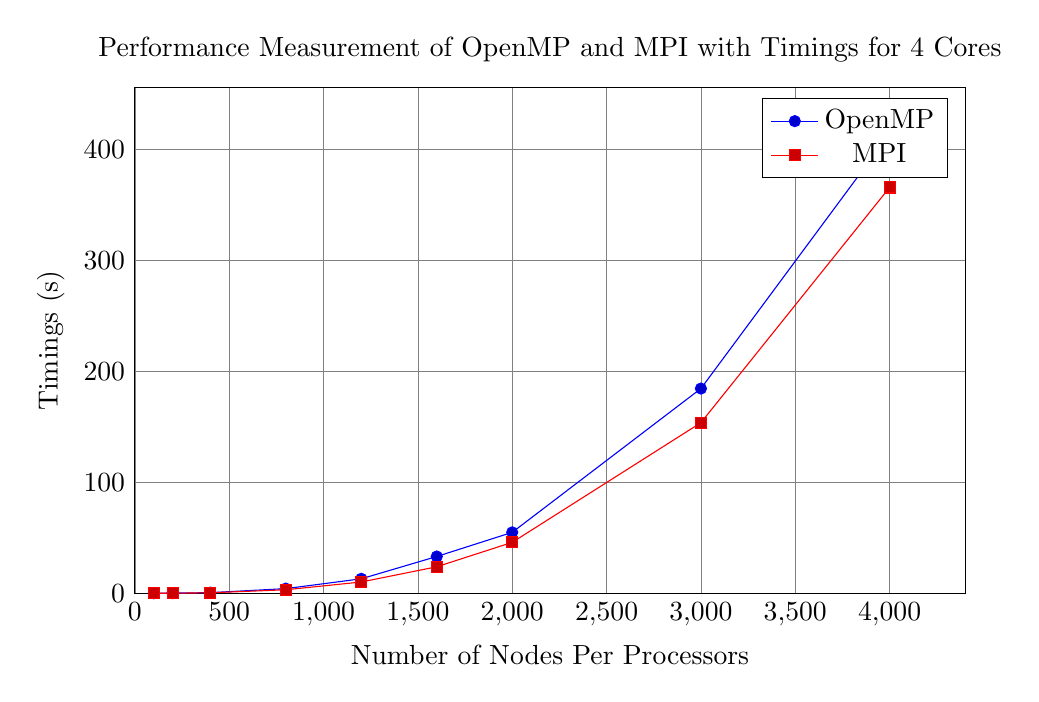
\begin{tikzpicture}
    \begin{axis}[
      width=1\linewidth, % Grafik genişliği belirle
      height=8cm, % Grafik yüksekliği belirle  
      ylabel={Timings (s)},
      xlabel={Number of Nodes Per Processors},
      grid=major, 
      ymin=0,
      xmin=0,
      grid style={help lines},
      title={Performance Measurement of OpenMP and MPI with Timings for 4 Cores},
    ]
    \addplot coordinates {
        (100,0.037792)
        (200,0.119862)
        (400,0.561629)
        (800,4.180215)
        (1200,13.032452)
        (1600,33.134146)
        (2000,54.880581)
        (3000,184.444051)
        (4000,413.980968)
    };
    \addlegendentry{OpenMP};

    \addplot coordinates {
        (100,0.013697)
        (200,0.068976)
        (400,0.420909)
        (800,3.156628)
        (1200,10.152554)
        (1600,23.874677)
        (2000,45.870164)
        (3000,153.687673)
        (4000,365.671162)
    };
    \addlegendentry{MPI};
    
    \end{axis}
  \end{tikzpicture}
  \caption{Performance Measurement of OpenMP and MPI with Timings for Fix Core Number(4)}
  \label{t1}
\end{figure}

\clearpage


\subsection{Results of Comparison the Number of Processes}
Similar to the trend in \ref{t1}, for varying number of processes, both MPI and OpenMP have the similar trend, which is uprising. However, as the number of processes increase, the gap between these two also increases in terms of timings. Considering this phenomenona, OpenMP is slower here also. 
\begin{figure}[hbt!]
  \centering
  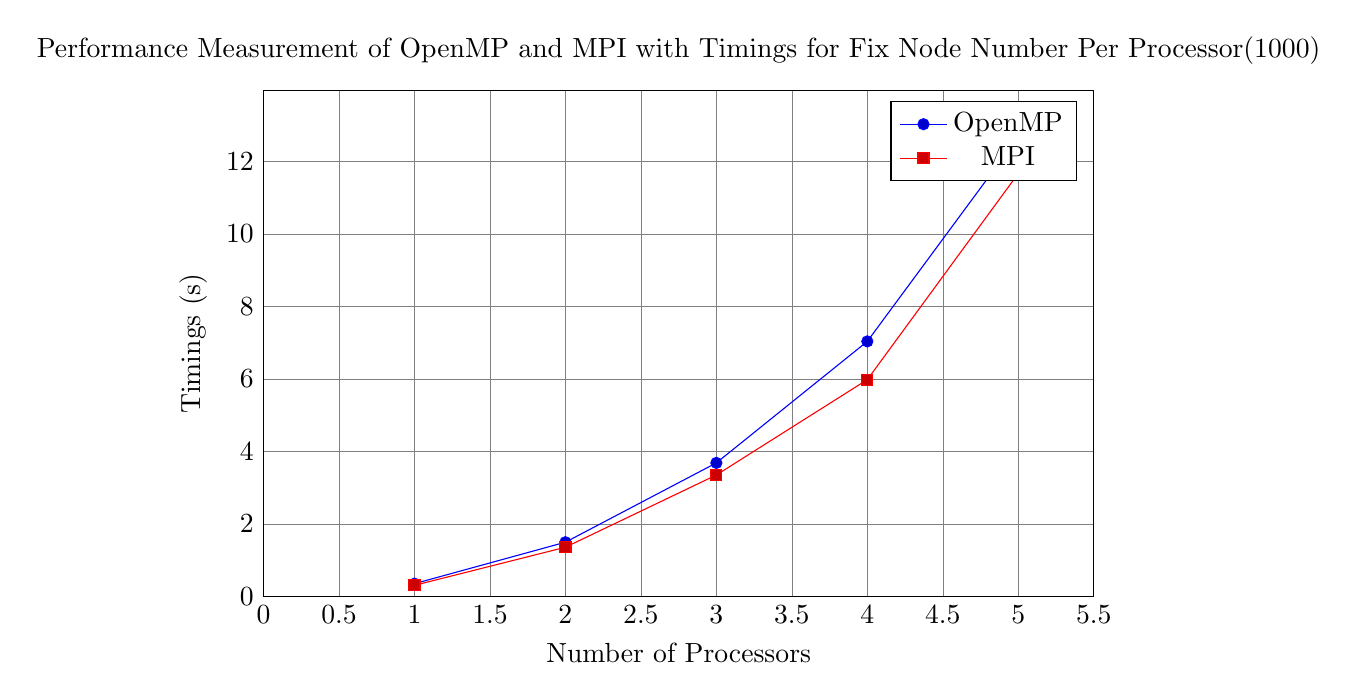
\begin{tikzpicture}
    \begin{axis}[
      width=1\linewidth, % Grafik genişliği belirle
      height=8cm, % Grafik yüksekliği belirle  
      ylabel={Timings (s)},
      xlabel={Number of Processors},
      grid=major, 
      ymin=0,
      xmin=0,
      grid style={help lines},
      title={Performance Measurement of OpenMP and MPI with Timings for Fix Node Number Per Processor(1000) },
    ]
    \addplot coordinates {
        (1,0.349737)
        (2,1.493712)
        (3,3.682316)
        (4,7.035118)
        (5,12.677928)
    };
    \addlegendentry{OpenMP};

    \addplot coordinates {
        (1,0.303556)
        (2,1.354715)
        (3,3.348535)
        (4,5.979146)
        (5,11.668409)
    };
    \addlegendentry{MPI};
    
    \end{axis}
  \end{tikzpicture}
  \caption{Performance Measurement of OpenMP and MPI with Timings for the Changing Processor Number}
  \label{t2}
\end{figure}

\clearpage

\subsection{Strong Scaling Analysis}
In strong scaling study, the problem size is kept fixed and the time for different number of processes is measured. As expected, increasing the number of processes decreases the required time since the node numbers per processor decreases. Here it is also observed that OpenMP is slower than MPI. 

\begin{figure}[hbt!]
  \centering
  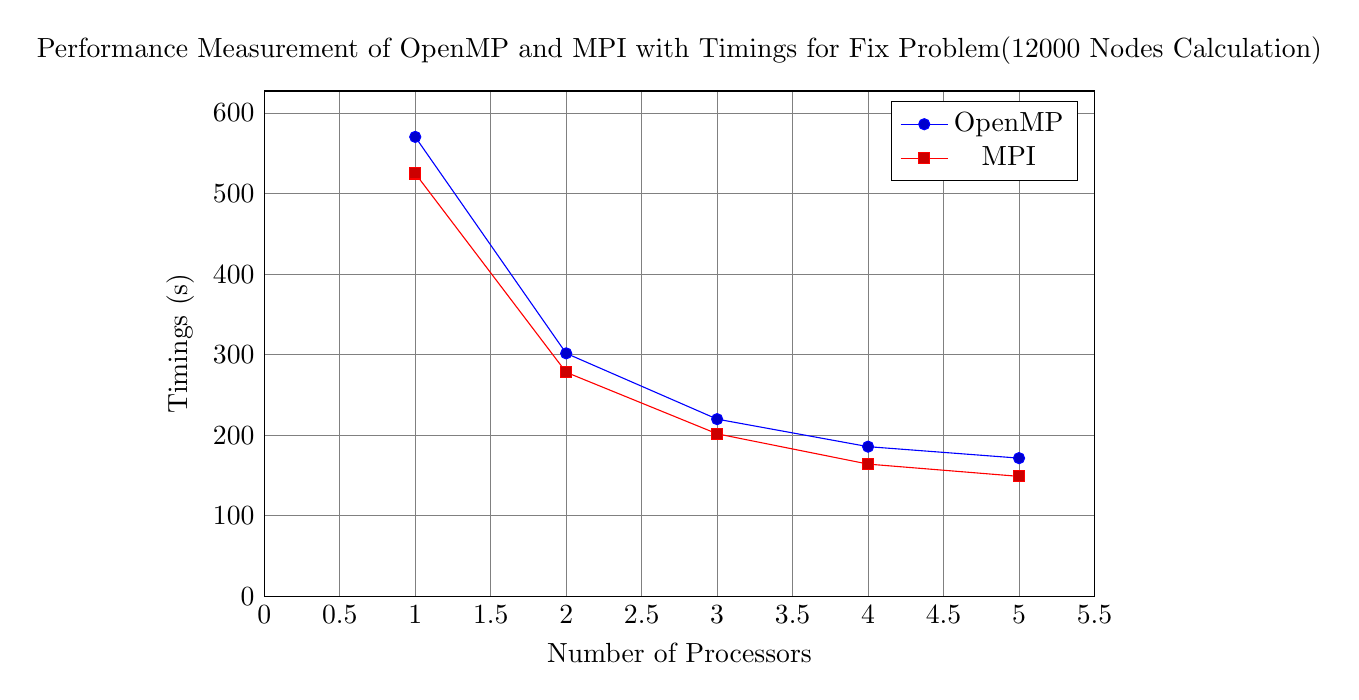
\begin{tikzpicture}
    \begin{axis}[
      width=1\linewidth, % Grafik genişliği belirle
      height=8cm, % Grafik yüksekliği belirle  
      ylabel={Timings (s)},
      xlabel={Number of Processors},
      grid=major, 
      ymin=0,
      xmin=0,
      grid style={help lines},
      title={Performance Measurement of OpenMP and MPI with Timings for  Fix Problem(12000 Nodes Calculation)},
    ]
    \addplot coordinates {
        (1,570.292419)
        (2,301.599327)
        (3,219.941292)
        (4,185.788597)
        (5,171.542332)
    };
    \addlegendentry{OpenMP}; 
    \addplot coordinates {
        (1,524.931910)
        (2,278.099906)
        (3,201.711407)
        (4,164.135979)
        (5,148.895396)
    };
    \addlegendentry{MPI};


    
    \end{axis}
  \end{tikzpicture}
  \caption{Performance Measurement of OpenMP and MPI with Timings for Strong Scaling Analysis}
  \label{t3}
\end{figure}

\clearpage

\section{Comments and Conclusion}


As seen in figures \ref{t2}, the timing increases dramatically with the number of nodes per cores. This is the expected result. Because when Nstep is calculated, sqrt of  (the total core number*node per core) is used.

As seen in figures \ref{t2}, the timing increases dramatically with the number of cores. This is the expected result. Same thing happen in this calculation too.  Because when Nstep is calculated, sqrt of  (the total core number*node per core) is used. 

As seen in figures \ref{t3}, the timing decreases with number of core for fixed problem. But this is not fully linear because of unparallel part and communication. 



\clearpage

\printbibliography

\end{document}
